\part{DiScholEd, une application développée avec le CMS TEI Publisher}

\chapter{Les corpus de DiScholEd }

Originellement, l'application présentait deux collections: les lettres et textes des intellectuels berlinois et la correspondance de Paul d’Estournelles de Constant. DiScholed possède en septembre 2023 sept corpus que l'on peut regrouper dans deux catégories différentes : les corpus du XIX\up{e} siècle et les corpus du XX\up{e} siècle. Les corpus sont en français, tchèque, allemand, anglais, hongrois, yiddish, latin, grec et italien.

\section{Les corpus XIX\up{e} siècle}

\subsection{Lettres et textes : Le Berlin intellectuel des années 1800}

Ce corpus est composé de lettres et de textes d’une dizaine d’intellectuels berlinois du début du XIX\up{e} siècle, parmi lesquels August Boeckh (1785-1867), Adelbert von Chamisso (1781-1838) et Ludwig Tieck (1773-1853). Ces auteurs ont participé à la naissance du romantisme allemand, un mouvement littéraire qui valorise l’imagination, le sentiment et la nature. Ils ont également fréquenté les cercles intellectuels de Berlin, où ils ont échangé leurs idées et leurs œuvres. Ce corpus illustre la diversité et la richesse de la culture allemande à cette époque. Le corpus comprend des documents personnels, mais aussi des œuvres de fiction (nouvelles, pièces de théâtre) et des travaux scientifiques (thèse). Le corpus a déjà fait l’objet d’une édition et d’une publication\footcite{DiScholEdBerlinintellectualsCorrespondences}, mais il nécessitait une mise à jour et une migration vers une plateforme de publication plus pérenne.

\subsection{Journal des guerres napoléoniennes}

Le fonds \og{}Nachlass Böttiger, Carl August (1760-1835) Saxonica und Sammlungen zur Zeitgeschichte\fg{}\footcite{bottigerNachlassBottigerCarl00} est un fonds d’archives conservé à la Bibliothèque d’État et Universitaire de Saxe (SLUB) à Dresde. Il contient le legs de Carl August Böttiger (1760-1835), un écrivain, journaliste et archéologue allemand, qui fut proche des représentants de la \textit{Weimarer Klassik}, le mouvement littéraire et culturel allemand du XVIIIe siècle. Le fonds comprend 297 volumes et capsules, dont une grande partie est constituée d'échanges de lettres avec Böttiger, ainsi que des documents sur l’histoire de la Saxe et de l’Allemagne.
    
Le corpus sur DiScholEd contient le manuscrit intitulé \og{}\textit{Journal des événements de Leipzig du 10 octobre [1813]}\fg{}. Il est rédigé par Friedrich Rochlitz (1769-1842) un écrivain, librettiste, biographe et critique musical saxon. Il s'agit d'un témoignage historique sur la bataille de Leipzig, qui opposa les armées de Napoléon à celles de la coalition formée par la Russie, la Prusse, l’Autriche et la Suède. Cette bataille se solda par une défaite française et marqua le début du déclin de l’Empire napoléonien. Le manuscrit relate les événements du 10 octobre 1813, jour où Napoléon lança une offensive contre les positions ennemies au sud de Leipzig.
    
\subsection{Correspondance de Constance de Salm (1767-1845)}

Constance de Salm (1767-1845) est une écrivaine française éminente de son époque. Originaire de Nantes, sous le nom de Constance Marie de Théis, elle publie ses premiers essais à 18 ans. Sa notoriété s'affirme en 1794 avec le livret du drame musical \og{}\textit{Sapho}\fg{}. Elle laisse derrière elle de nombreux poèmes et panégyriques acclamés, ainsi qu'un roman intitulé \og{}\textit{Vingt-quatre heures de la vie d'une femme sensible}\fg{}. Ses œuvres abordent des enjeux socio-politiques contemporains, notamment l'éducation des femmes et leur place dans la société. Constance de Salm est la première femme admise au sein du cercle de l'Athénée des arts à Paris, une association regroupant artistes et érudits. À travers son salon parisien, elle réunit un cercle prestigieux d'amis, parmi lesquels des écrivains, des chercheurs et des artistes éminents de son temps. Cette correspondance étendue est menée de front avec ces personnalités.

Le corpus de lettres de Constance de Salm est composé d'environ 11 000 lettres et documents conservés dans deux archives distinctes (le fond \og{}Salm\fg{} de la Société des Amis du Vieux Toulon et de sa Région et d'autre part de la collection \og{}Constance de Salm\fg{} des archives du \og{}Schloss Dyck\fg{} de la \og{}\textit{Vereinigte Adelsarchive im Rheinland e.V.}\fg{}). Ces documents sont divisés en deux parties principales : les transcriptions que Constance de Salm a faites de son vivant pour préparer l'édition de sa correspondance et les lettres originales. Datant principalement des années 1798 à 1844, ce corpus regroupe environ 350 auteurs et destinataires variés. Le contenu de ces lettres offre une perspective unique sur la vie littéraire et scientifique à Paris pendant cette période. Ces documents éclairent les enjeux et les conditions de l'écriture féminine, tout en illustrant les mécanismes des réseaux et des échanges culturels entre le Rhineland et la France au XIXe\up{e} siècle.

\subsection{August Boeckh - Catalogue de ses manuscrits}

August Boeckh, philologue classique (1785-1867) est connu pour l'histoire des sciences et la politique scientifique. Au sein de l'Académie des sciences de Prusse, Boeckh a promu la recherche scientifique en lançant des projets d'envergure, notamment le projet du \og{}\textit{Corpus Inscriptionum Graecarum}\fg{}. À partir de 1811, il a entamé sa carrière d'enseignant à l'université de Berlin, où il a également contribué à façonner la structure de l'institution. Il occupe alors les postes suivants: doyen de la faculté des arts et des sciences humaines, recteur de l'université, et fondateur du séminaire philologique en 1812.

Le projet Boeckh Nachlassprojekt a été créé pour cataloguer les manuscrits rédigés de la main d'August Boeckh lui-même ou dans lesquels il a laissé une marque significative. Cette collection comprend une grande quantité de documents issus de ses nombreuses activités en tant que doyen, président de diverses commissions et directeur du séminaire philologique à l'université de Berlin entre 1811 et sa disparition en 1867. \footcite{DiScholEdBerlinintellectualsCorrespondences}

\section{Les corpus XX\up{e} siècle}

\subsection{Correspondance de d'Estournelles de Constant}

Ce corpus regroupe les échanges de Paul d’Estournelles de Constant (1852-1924), diplomate et homme politique français, avec Nicholas Murray Butler, universitaire et homme politique américain. Ces deux hommes, lauréats du prix Nobel de la paix (en 1909 pour Paul d’Estournelles de Constant et 1931 pour Nicholas Murray Butler), ont entretenu une relation épistolaire régulière entre 1914 et 1924. Ils ont partagé leurs expériences, leurs opinions et leurs sentiments sur le conflit, tout en défendant leur idéal pacifiste et leur projet d’organisation mondiale. Ce corpus présente un intérêt historique et littéraire, car il s’agit de documents personnels qui témoignent à la fois de la vie quotidienne et des enjeux politiques de l’époque. Le corpus est également riche, puisqu’il comprend environ 1500 lettres, de longueur variable, rédigées à la machine à écrire.

\subsection{Ma Guerre 1914-1918}

Charles Bruneau (1883-1969) est un linguiste français, spécialiste de la langue française et de la littérature médiévale. Pendant la Première Guerre mondiale, il est mobilisé comme soldat et participe aux combats sur le front occidental. Il écrit plus de 600 lettres à sa femme et à sa famille, ainsi qu’un journal personnel, où il relate son expérience de la guerre, ses souffrances, ses espoirs et ses réflexions. De ces écrits, il tire un ouvrage intitulé \textit{Ma guerre 1914-1918}, composé d’extraits classés, datés et situés par l’auteur, qui témoignent de sa vision de la guerre et de son évolution personnelle. Ce manuscrit, resté inédit jusqu’en 2018, a été publié par les éditions Terres Ardennaises, avec la collaboration de Nicolas Beaupré, Michel Tamine (Institut Charles-Bruneau) et Jacques Lambert (Terres Ardennaises)\footcite{MaGuerre19141918}. Il constitue un document historique et littéraire de grande valeur, qui révèle le regard d’un intellectuel sur le conflit mondial et sur la langue française. Notre corpus possède aussi une annexe qui est le journal de son oncle Raymond Bruneau, demeuré à Givet durant la guerre, au chevet de son père.

\subsection{Premiers témoignages sur l'Holocauste}

Le corpus “Premiers témoignages de l’Holocauste” est un projet qui vise à rassembler, analyser et diffuser des témoignages écrits et oraux de survivants de l’Holocauste recueillis peu après la fin de la Seconde Guerre mondiale. Il s’agit d’une collaboration entre plusieurs institutions européennes, dont l’Institut d’histoire contemporaine de Munich, le Mémorial de la Shoah de Paris et le Wiener Holocaust Library de Londres. Le corpus comprend des documents en plusieurs langues, notamment l’allemand, le français, l’anglais et le yiddish. Il offre un accès à des sources historiques uniques et précieuses pour comprendre les expériences et les réactions des victimes du génocide nazi. \\

DiScholed dispose de sept corpus multilingues, tous encodés en XML conformément aux normes de la TEI (Text Encoding Initiative). Afin de les rendre accessibles en ligne, il a été décidé d'opter pour un système de gestion de contenu (CMS).

\chapter{Les CMS et TEI Publisher}

Les CMS (\textit{Content Management System}) comme TEI Publisher sont des programmes informatiques qui permettent de créer un site ou une application. Ils présentent de nombreux avantages qui facilitent considérablement le déploiement d'application. TEI Publisher est un CMS spécialement dédié aux éditions numériques. 

\section{Présentation des CMS}

Les CMS les plus connus\footcite{MeilleurCMS2023} sont \href{https://fr.wordpress.org/}{WordPress\footcite{WordPress}} ou encore \href{https://fr.wix.com/}{Wix\footcite{Wix}}. Les CMS sont aujourd'hui des références pour la création et le déploiement rapide de sites, tant pour des particuliers que pour des entreprises. 
Cette explosion\footcite{CMSOpenSource} de la popularité des CMS s'explique par le fait qu'utiliser un CMS présente de nombreux avantages. Grâce à cet outil, il est possible de considérablement réduire le temps nécessaire au développement d'un site.

Le CMS offre aussi la possibilité de développer des applications Web. En mettant à disposition une variété de \textit{plugins}, le système de gestion de contenu facilite la création d'un site sans que l'éditeur ait à se soucier du codage.

Un autre atout du CMS est son intégration native d'un créateur de page, ou \textit{page builder}, qui permet de créer, de gérer et de modifier facilement le contenu du site en utilisant des blocs dynamiques réutilisables.

La sécurité est également un point fort des CMS, car ils proposent des fonctionnalités avancées pour protéger le contenu et la base de données du site contre les tentatives d'intrusion. L'auteur du site peut aussi gérer les accès et les autorisations à l'aide des systèmes de gestion des rôle et des droits des comptes utilisateurs directement intégrés avec le CMS.

Le référencement SEO (Search Engine Optimization)  est l'ensemble des pratiques visant à optimiser la visibilité d'un site Web dans les résultats organiques des moteurs de recherche. Les CMS sont aussi optimisés pour améliorer la visibilité avec le SEO. 

Enfin, un CMS offre de meilleures possibilités de gestion et de relation utilisateur. Des fonctionnalités telles que les formulaires de contact et le chat en direct sont intégrées pour répondre aux demandes urgentes des utilisateurs.

Les chercheurs en SHS (Sciences Humaines et Sociales) ont des besoins divers en matière de gestion de contenu, que ce soit pour publier des articles, des documents de recherche, ou pour créer des plateformes collaboratives. Les CMS offrent des solutions pour toutes ces tâches.\\

Les multiples avantages qu'offre un système de gestion de contenu (CMS) sont la principale raison du choix d'opter pour cette solution. DiScholed a spécifiquement choisi TEI Publisher, un CMS spécialement conçu pour les éditions numériques, en raison de ses caractéristiques particulières.

\section{TEI Publisher}

TEI Publisher est toujours en développement et reçoit des mises à jour majeures deux fois par an, apportant de nouvelles fonctionnalités et corrigeant les \textit{bugs}. L'objectif est de permettre aux chercheurs et aux éditeurs de publier leurs documents rapidement, facilement et avec des compétences minimales en programmation. 

TEI Publisher est une application open source pour eXist-db (une plateforme de développement pour les applications basées sur XML). Elle est compatible avec les documents TEI (Text Encoding Initiative) tout en offrant la possibilité d'être adaptée à n'importe quel autre schéma\footcite{AtomicWiki}. Elle permet de publier une édition numérique sans écrire de code. En utilisant le modèle de traitement TEI, la personnalisation de l’apparence du texte se fait entièrement en XML. TEI Publisher produit des applications qui intègrent déjà des fonctionnalités telles que la navigation page par page, la fonction de recherche, et la possibilité d'exporter vers différents formats.\footcite{TEIPublisherDocumentation}

TEI Publisher est un projet collaboratif basé sur les idées et les contributions du monde entier. Il a été initialement inspiré par la vision derrière le modèle de traitement TEI \og{}travail du défunt Sebastian Rahtz et d’autres membres du projet TEI Simple de 2015\fg{}\footcite{TEIPublisher} et continue d’évoluer. Il est sous licence GPLv3 et fonctionne grâce à Exist-db.

Exist-db simplifie grandement la gestion du \textit{back-end}, qui fait référence à la partie invisible d'une application informatique, celle qui gère les données, les processus et la logique sous-jacente. Contrairement à l'interface utilisateur visible du logiciel (appelée le \textit{front-end}), le back-end travaille en coulisses pour garantir le bon fonctionnement de l'application. Pour gérer le \textit{back-end} plusieurs logiciels sont fournis avec exist-db:

\begin{itemize}[label=\textbullet]
    \item eXide - XQuery IDE : eXide est un environnement de développement intégré (IDE) pour XQuery qui permet de développer et de déboguer des applications XQuery pour eXist-db.
    \item eXist-db Demo Apps : Les applications de démonstration d’eXist-db montrent comment utiliser les fonctionnalités d’eXist-db pour créer des applications Web.
    \item eXist-db Documentation : La documentation d’eXist-db fournit des informations détaillées sur l’utilisation et la configuration d’eXist-db, ainsi que sur les fonctionnalités et les API (\textit{Application Programming Interface} ou \og{}Interface de Programmation Applicative\fg{} est un ensemble de règles et de protocoles permettant à l'application de communiquer et d'échanger des données avec le serveur) disponibles.
    \item Monex : Monex est un outil de surveillance et de gestion de performances pour eXist-db qui permet de surveiller les performances du serveur et de diagnostiquer les problèmes.
    \item XQuery Function Documentation : La documentation des fonctions XQuery fournit une référence complète des fonctions XQuery disponibles dans eXist-db.
\end{itemize}

La documentation officielle de TEI Publisher se décrit comme: \og{}un outil qui permet aux chercheurs et aux éditeurs de publier leurs travaux sans devenir des programmeurs, tout en ne les contraignant pas à un cadre universel. Les développeurs expérimentés en bénéficieront également\fg{}\footcite{TEIPublisher}. Pour aider les non-programmeurs, TEI Publisher a fait d'intégrer le \textit{low-code} avec la mise en place d'une interface graphique pour modifier l'ODD et des fonctionnalitées déjà fonctionnelles dans les applications.
C'est pourquoi TEI Publisher semble être un choix idéal pour DiScholed : il offre des restrictions suffisantes pour protéger l'application tout en offrant une certaine liberté pour gérer un projet aussi vaste. Avec ses sept corpus, DiScholed requiert un CMS spécialisé pour élaborer une application fonctionnelle et novatrice. \\

Afin de déterminer si TEI Publisher convient à DiScholed, il est nécessaire d'analyser les problèmes (\textit{bugs}) survenus lors du développement de l'application. Il s'agit ensuite de déterminer si ces erreurs peuvent être résolues par des personnes n'ayant pas de compétences en développement, et si TEI Publisher tient sa promesse d'être un CMS accessible à tous.

\chapter{Les \textit{bugs} de DiScholEd}

L'application DiScholEd à chaque ajout d'un nouveau corpus présentait de nouveaux problèmes/défis. En septembre 2023 on compte une quinzaine de problèmes répertoriés sur le GitLab de l'entreprise. 
Pour éviter de générer des \textit{bugs}, les CMS ont la possibilité de choisir entre une approche restrictive ou une approche plus libre.

\section{La fiabilité des CMS : prévention et correction des erreurs}

Un CMS peut varier considérablement en termes de restrictions ou de liberté en fonction de plusieurs facteurs. L'une des principales raisons pour lesquelles un CMS peut être très restrictif est liée à son objectif initial. Certains CMS sont conçus pour des utilisations spécifiques et ont des modèles de données, des structures de page et des fonctionnalités prédéfinis, ce qui limite la personnalisation. Ces CMS sont souvent adaptés à des besoins spécifiques, tels que la création de blogs ou de sites de commerce électronique, et ils peuvent imposer des contraintes pour maintenir la cohérence et la sécurité.

En revanche, les CMS plus libres sont souvent des systèmes open source qui permettent une personnalisation étendue. Ils offrent une flexibilité presque illimitée pour la conception de sites Web, ce qui en fait un choix populaire pour les projets complexes et personnalisés. Les utilisateurs peuvent créer leurs propres modèles, ajouter des fonctionnalités sur mesure et adapter le CMS à leurs besoins spécifiques. Cependant, cette liberté peut également entraîner une complexité accrue et nécessiter des compétences de développement plus avancées pour tirer pleinement parti du potentiel du CMS.

Ainsi, le choix entre un CMS restrictif et un CMS libre dépend des besoins et des compétences de l'utilisateur, ainsi que de l'objectif du projet. Un CMS restrictif peut être idéal pour les projets simples, tandis qu'un CMS libre offre une plus grande marge de manœuvre pour les projets complexes, mais nécessite souvent un investissement en termes de temps et de connaissances techniques. \\

Pour DiScholEd, nous avons besoin d'un CMS assez libre pour nous permettre de bien présenter nos sept corpus, mais un CMS restrictif pour éviter de créer trop de \textit{bugs} car il n'y a pas de développeur expérimenté sur le projet. TEI Publisher comme nous l'avons défini est un entre-deux entre un CMS libre et restrictif.
\section{TEI Publisher et sa gestion des erreurs}
TEI Publisher permet avec des documents XML et des templates HTML de générer des pages web. Tous les \textit{bugs} peuvent être alors réglés en modifiant l'ODD ou les \textit{templates} HTML. Une ODD fait référence à \textit{One Document Does it all}, qui est une approche pour décrire la structure, le contenu et les contraintes d'un document XML. Pour modifier l'ODD, il est possible d'utiliser l'interface graphique de TEI Publisher directement depuis l'application. Le logiciel eXide permet aussi d'accéder aux fichiers de l'application, dont l'ODD et les templates.

\subsection{L'ODD}

L'ODD est la principale source de bug pour les applications TEI Publisher, c'est pourquoi une interface graphique a été créée par TEI Publisher nous empêchant de créer un code défectueux (cf Figure \ref{fig:schémas04}). Depuis l'interface des messages d'erreurs ou des menus déroulant nous permettent de crééer une ODD fonctionnelle.

\newpage

 \begin{figure}[H]
        \centering
        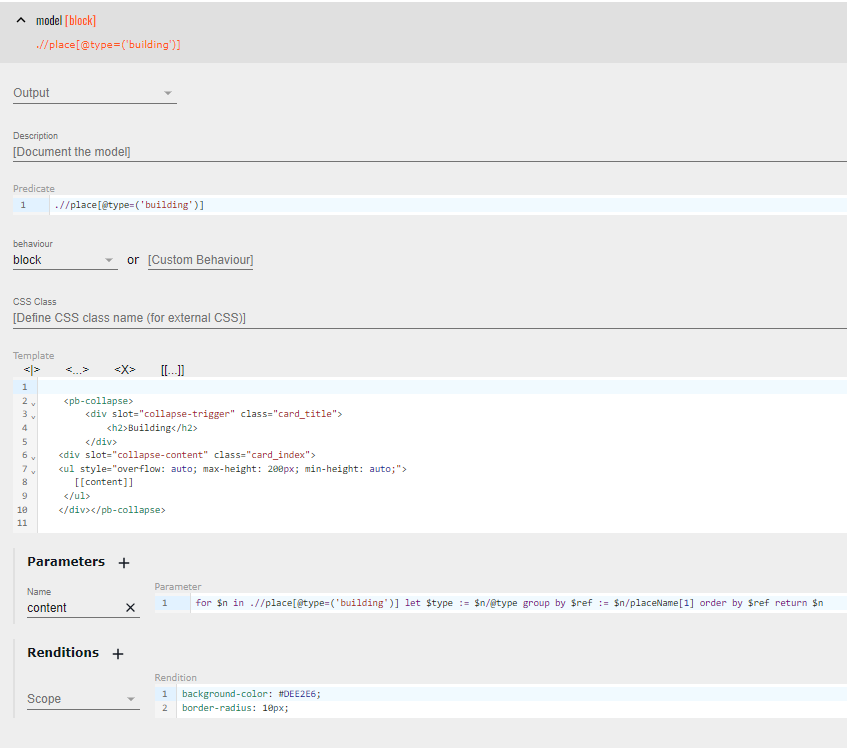
\includegraphics[width=0.75\linewidth]{schémas/building_places.png}
        \caption{Exemple de déclaration d’un élément dans l’interface graphique de l’ODD}
        \label{fig:schémas01}
    \end{figure}

Cependant, une ODD peut devenir inutile si elle n'est pas adaptée aux encodages spécifiques des fichiers XML que nous utilisons. DiScholEd contient sept collections provenant d'institutions différentes, et bien qu'elles respectent globalement les normes et directives de la TEI, certaines différences subsistent et peuvent perturber la conformité de l'ODD. Le problème ne viendra pas alors de TEI Publisher mais de notre ODD et/ou de l'encodage des corpus.

\subsection{Les templates HTML}

TEI Publisher, dans sa documentation, explique que pour produire une application, seules des compétences en HTML sont requises. C'est en effet nécessaire pour pouvoir utiliser les composants du \textit{Bundle} JavaScript (une librairie de balises HTML personnalisées). L'un des principes fondamentaux de TEI Publisher est de réutiliser et de partager les solutions ou idées des templates. Ainsi, les applications se ressemblent très souvent car elles proviennent du même ensemble de modèles, comme le montrent les figures suivantes (cf Figure \ref{fig:schémas02} et Figure \ref{fig:schémas03}):

\begin{figure}[H]
\centering
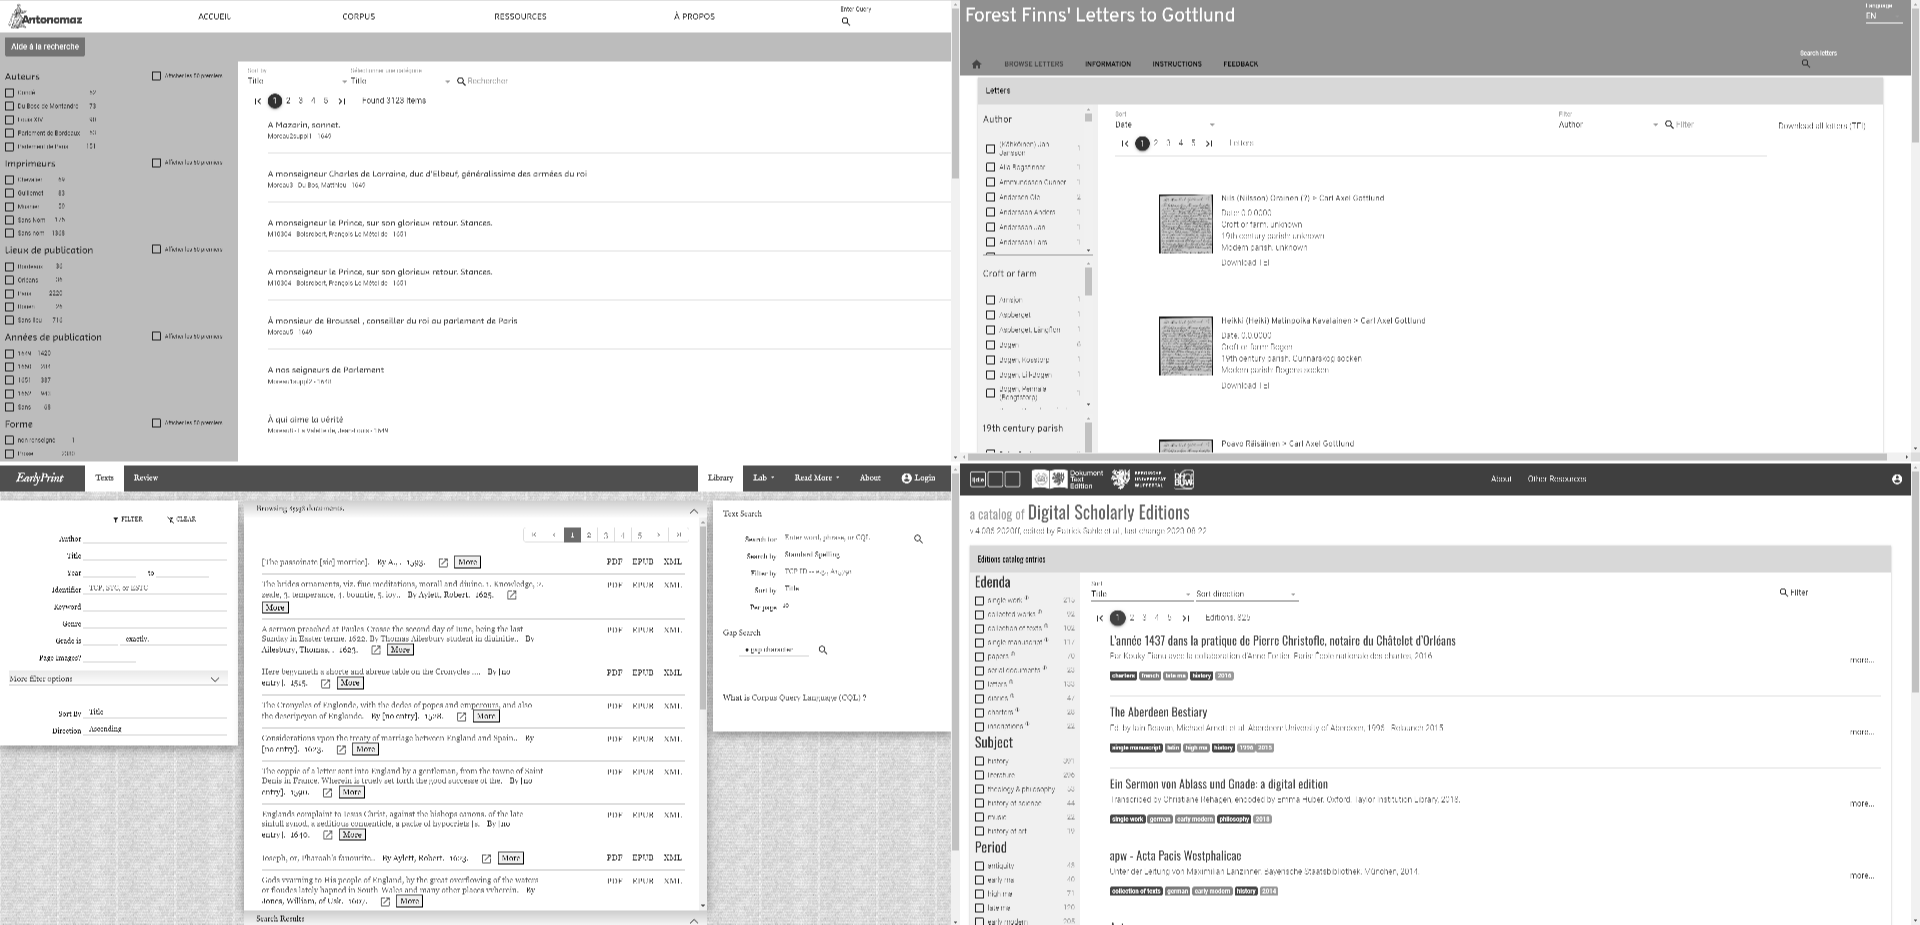
\includegraphics[width=1\linewidth]{schémas/4_webtei-modified.png}
\caption{Capture d'écran de 4 sites différents créés avec TEI Publisher (Antonomaz, Forest's Finn's Letter to Gottlund, Digital Scholarly Edition et EarlyPrint) }
\label{fig:schémas02}
\end{figure}

\begin{figure}[H]
\centering
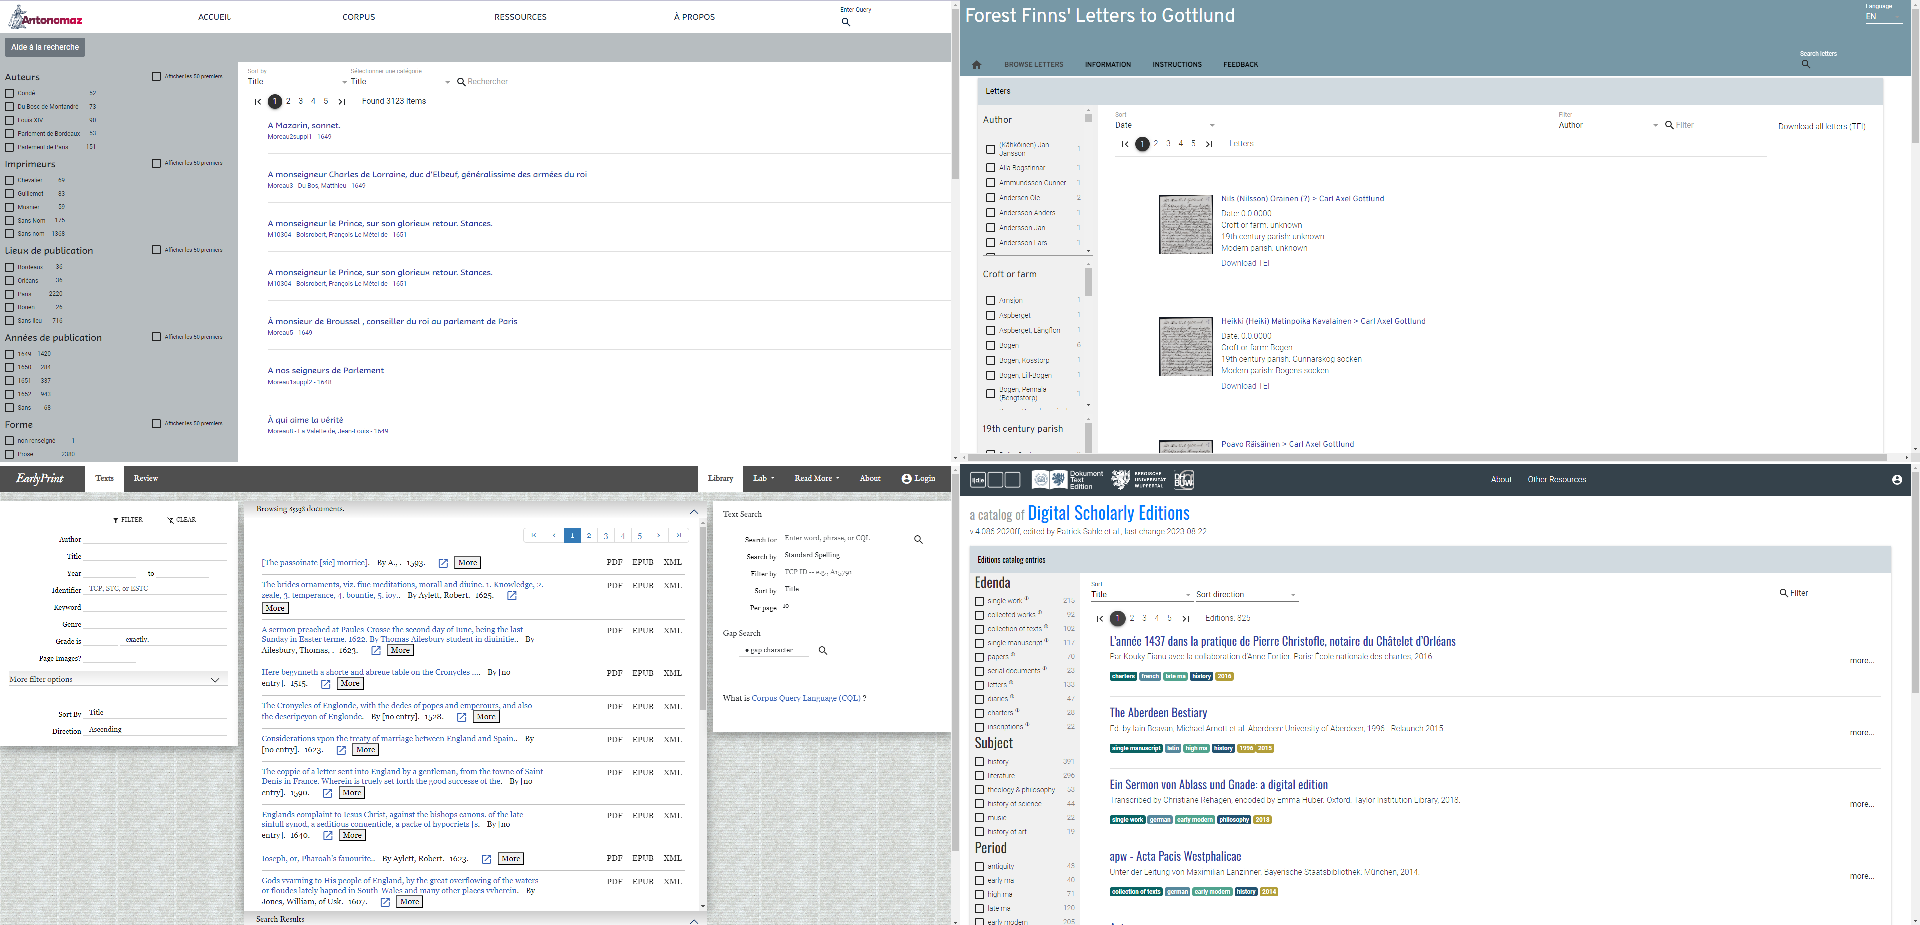
\includegraphics[width=1\linewidth]{schémas/4_webtei.png}
\caption{Capture d'écran des 4 sites avec leurs couleurs respectives (Antonomaz, Forest's Finn's Letter to Gottlund, Digital Scholarly Edition et EarlyPrint)}
\label{fig:schémas03}
\end{figure} 

La plupart de ces applications est souvent accessible sur Internet, avec une documentation complète de tous les composants disponibles sur \href{https://cdn.tei-publisher.com/@2.11.1/dist/api.html}{le site officiel}\footnote{\textit{TEI Publisher Webcomponents API}, URL: https://cdn.tei-publisher.com/@2.11.1/dist/api.html (visité le 29/08/2023)} de TEI Publisher.

TEI Publisher, en cherchant à offrir une grande liberté et à rendre la publication accessible aux non-codeurs, peut parfois générer des problèmes. Cette liberté peut désorienter les utilisateurs inexpérimentés, les amenant à prendre des décisions qui peuvent entraîner des erreurs. En d'autres termes, la flexibilité de TEI Publisher peut parfois se traduire par des erreurs, car elle permet aux utilisateurs de faire ce qu'ils veulent, même si cela ne correspond pas nécessairement aux meilleures pratiques en matière de développement.\\

Pour résumer, le projet DiScholed possède des corpus qui présentent tous un intérêt historique et a besoin d'un CMS pour les déployer sur Internet. Il existe beaucoup de CMS qui sont tous développés pour créer des applications bien spéciales. TEI Publisher, un CMS dédié aux éditions numériques et qui se veut accessible à tous, devrait être une solution pour notre projet. Le CMS parfait pour notre projet est assez libre pour nous permettre de mettre chaque corpus en avant et est assez restrictif pour nous évitez de détruire l'application. Nous avons identifié d'où pourraient provenir les \textit{bugs} générés par TEI Publisher, mais il nous faut maintenant examiner en détail ceux de DiScholed spécifiquement. En étudiant les \textit{bugs} de DiScholed, il sera alors possible de déterminer si TEI Publisher peut convenir à notre projet.